\documentclass[12pt]{report}
\usepackage[utf8]{inputenc}
\usepackage[french]{babel}
\usepackage[T1]{fontenc}
\usepackage{amsmath}
\usepackage{amsfonts}
\usepackage{amssymb}
\usepackage{graphicx}
\usepackage{titlesec}
\usepackage{caption}
\usepackage{titling}
\usepackage{booktabs}
\usepackage{enumitem}
\usepackage{eurosym}
\usepackage{epigraph}
\usepackage{hyperref}
\usepackage{fontspec}
\usepackage{ragged2e}
\usepackage{parskip}
\usepackage{wrapfig}
\usepackage{calc}
\usepackage{float}

\graphicspath{ {img/} }
\setlength{\droptitle}{-10em}
\titleformat{\chapter}[hang]{\normalfont\huge\bfseries}{\thechapter. }{0em}{}

\begin{document}

\title{
	{\Huge Projet OCR}\\
	\vspace{2em}
	{\Huge Rapport de soutenance}\\
	{\large Wizard Neurons}
}
\author{
	Antoine Gonzalez\\
	Cédric Parpet
	\and
	Louis Le-Gatt\\
	Jérémy Salfati}
\date{
	\vspace{15em}
	{Dossier Projet Informatique\\
	Info-Spé EPITA\\
	Octobre 2018}
}

\maketitle
\newpage
\newpage
\tableofcontents

\chapter{Introduction}

Cette première moitié de projet aura été assez difficile, mais très intéressante. N'ayant eu que peu de cours de C, il nous a fallu apprendre par nous même tout ce dont nous avions besoin. De plus, ce projet nous laisse bien moins de libertés que celui du semestre précédent, plus de limites nous sont imposées, tant sur le projet lui-même que sur la manière de l'implémenter. Ce qui nous force à chercher des solutions parfois moins évidentes.

Cependant, le groupe est motivé: un OCR est très intéressant à mettre en place et nous permet de nous essayer à beaucoup de concepts différents de la programmation: l'interface utilisateur avec GTK, le traitement d'image avec la SDL, et enfin l'intelligence artificielle (buzzword du moment) avec les réseaux de neurones. Et surtout, le langage C qui nous a été imposé est un classique de la programmation, et apprendre à l'utiliser nous permettra de mieux saisir certains concepts de la programmation avec deslangages plus haut-niveaux, et de comprendre par exemple la gestion de la mémoire.

C'est donc avec soif de connaissances que nous nous sommes mis au travail, en quête du meilleur OCR réalisable. Durant ces premières semaines, chacun a pu expérimenter avec sa partie. Nous possédons désormais les connaissances et outils nécéssaires à la bonne réalisation du projet.

Dans ce rapport, nous allons présenter notre vision du projet ainsi que les avancées que nous avons réalisé, les difficultés rencontrées, et enfin nos plans pour la seconde soutenance.

\begin{figure}
    \centering
    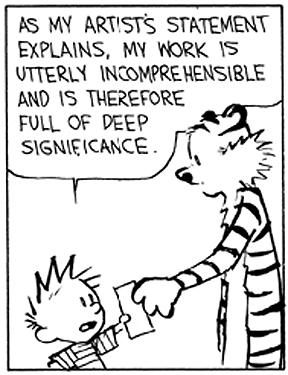
\includegraphics[width=0.6\textwidth]{project_mood_S1}
    \caption*{\textit{Calvin and Hobbes}, Bill Watterson}
\end{figure}

\chapter{Répartition des tâches}

Afin de rester organisés tout au long de ce projet, nous nous sommes réparties les tâches de la manière suivante.

\begin{center}
    \begin{tabular}{@{} l *4c @{}}
        \toprule
        \multicolumn{1}{c}{}    & \textbf{Antoine}  & \textbf{Louis}  & \textbf{Cédric} & \textbf{Jérémy} \\ 
        \midrule
        Chargement de l'image & & & & X \\
        Traitement de l'image & & X & & \\
        Découpage de l'image & & & X & \\
        Réseau Neuronal & X & & & \\
        Sauvegarde des résultats & & & & X \\
        Interface Utilisateur & & & & X \\
        \bottomrule
    \end{tabular}
\end{center}


En somme, Antoine s'occupera de tout ce qui touchera de près ou de loin au réseau de neurones. Louis se chargera du traitement primaire des images (black\&white ou grayscale, création d'une toolbox pour la manipulation des pixels...). Cédric devra s'occuper du découpage de l'image en lignes puis caractères, et de la reconstruction du texte reconnu par le réseau de neuronnes. Enfin, Jérémy sera en charge de l'interface utilisateur, afin de pouvoir utiliser tous nos systèmes de manière intuitive.

Bien entendu, chaque membre reste disponible pour aider les autres en fonction des besoins et du temps disponible.

\chapter{Diagramme Fonctionnel}

Afin que chaque membre comprenne parfaitement ce qui est attendu de sa partie et comment elle devra interagir avec celle des autres membres, nous avons réalisé un diagramme fonctionnel de l'OCR. On peut y voir le déroulement de son éxecution, du moment où l'utilisateur charge une image, au moment où le texte détecté est affiché et enrgistré \textit{(voir figure ci-dessous)}.

Comme on peut le voir, chaque partie interagit de manière simple avec le reste, et possède un but bien définit. Chaque morceau de l'OCR n'appelle qu'une unique autre partie, ce qui limite les erreurs potentielles d'appels croisés entre les multiples fonctions. Chaque membre du groupe n'a donc qu'à penser à une seule autre partie. Il lui suffit de spécifier quel type de valeur il attend en retour, et quel type de valeur il est capable d'envoyer. La partie suivante n'a qu'à s'adapter à ces règles, et faire de même.

\begin{figure}[H]
    \centering
    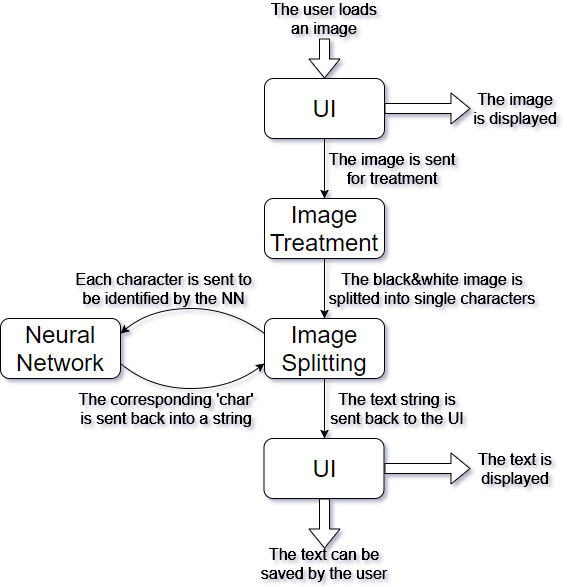
\includegraphics[width=1\textwidth]{OCR_functionnal_diagram}
    \caption{Functional diagram}
\end{figure}

\chapter{Avancement}

\section{Traitement de l'image (Louis)}

J’ai eu à charge la partie sur le traitement de l’image. J’ai ainsi décidé de commencer par travailler sur le chargement de l’image et sa sauvegarde. Pour cela je me suis renseigné sur « comment traiter une image en C ?» et « Quelles sont les outils pratique pour faciliter le travail sur les images en C ? ». J’ai très vite compris que j’allais devoir travailler à l’aide de la bibliothèque SDL qui permet le traitement des images de manière simple.
 
Nous avons ensuite décidé des différentes fonctions utiles pour les différents membres du groupe.
J’ai ensuite développé un programme permettant de tester mes fonctions en affichant l’image puis en l’actualisant après application des différentes fonctions. Tout ceci toujours grâce à la bibliothèque SDL qui permet d’afficher une image sur une fenêtre en quelques lignes seulement.

Ainsi en accord avec les membres du groupe et le livret j’ai décidé de réaliser plusieurs fonctions :

\newpage
\begin{itemize}[label=\textbullet]
	\item Une fonction qui supprime les couleurs d’une image afin d’obtenir une image en noir et blanc. Cette fonction utilise 2 autres fonctions vue en travaux pratiques : getpixel et putpixel qui permette pour la première de récupérer la valeur d’un pixel donné et pour l’autre de placer un pixel sur une surface à une coordonnée x,y choisie. J’ai ainsi décidé de placer ces fonctions dans un fichier à part des fonctions de traitement de l’image car celle-ci peuvent s’avérer utile pour les autres membres du groupe. Ces deux fonctions m’ont permis de récupérer la valeur du pixel et de la changer en noir ou en blanc en fonction de la couleur du pixel. Cependant après quelques discussions avec les autres membres du groupe nous avons décidé que l’image en noir et blanc n’était peut-être pas la meilleure solution pour le découpage et le réseau de neurones. Nous avons cherché une autre manière de supprimer les couleurs de l’image. La solution qui semble la mieux adapté pour les traitements à réaliser fut celle d’obtenir une image en teinte de gris (dis grayscale).
\end{itemize}
\begin{figure}[H]
    \centering
    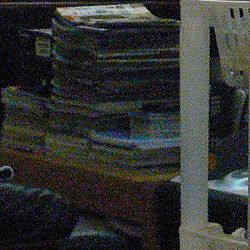
\includegraphics[width=0.5\textwidth]{noise}
    \caption{Original image}
\end{figure}

\newpage
\begin{itemize}[label=\textbullet]
	\item La deuxième fonction que j’ai alors réalisée fut une fonction permettant de encore une fois supprimer les couleurs et de cette fois ci les remplacer par leur teinte de gris associé. Il a donc fallu faire plusieurs recherches sur la teinte de gris la plus adapté pour notre travail. J’ai donc opté pour 3 coefficients appliqués aux valeurs du rouge, du bleu et du vert de chacun des pixels. Puis il suffit d’additionner ces trois valeurs (après multiplication par leur coefficient respectif) afin d’obtenir notre valeur de gris propre au pixel actuel. 
	\item J’ai ensuite réalisé une fonction de sauvegarde d’image permettant de sauvegarder les modifications de l’image. Puis une fonction de copie d’une image. Celle-ci sera très utile afin de ne pas réaliser tous ces traitements sur l’image que l’utilisateur va nous fournir. En effet nous souhaitons restituer à l’utilisateur son image sans aucun changement de nom ou de structure. 
\end{itemize}
\begin{figure}[H]
    \centering
    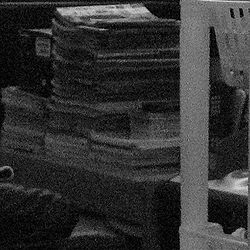
\includegraphics[width=0.5\textwidth]{grayscale}
    \caption{Grayscale}
\end{figure}

\newpage
\begin{itemize}[label=\textbullet]
	\item J’ai finalement décidé d’ajouter une fonctionnalité supplémentaire au traitement de l’image. En effet en testant mon code avec plusieurs images différentes je me suis très vite rendu compte de plusieurs defaults pouvant apparaitre sur l’image. J’ai fait quelques recherches qui m’ont conduit conclure qu’il s’agissait de « bruit ». J’ai alors décidé d’essayer de réduire au maximum ce bruit sur notre image afin de faciliter les étapes suivantes de notre OCR. Après de nombreuse recherche à travers des manières plus ou moins complexe de corriger ce bruit j’ai décidé de le réduire en utilisant un filtre médian. Ce filtre médian fonctionne de manière très simple. Il parcourt l’image pixel par pixel et observe pour chacun des pixels, ses pixels voisins. Il réalise ensuite une liste de ces différents pixels en y intégrant leur valeur numérique correspondant à leur couleur. Finalement cet algorithme trie cette liste en ordre croissant. La valeur médiane de cette liste devient alors la nouvelle valeur du pixel. Ainsi chaque pixel est une moyenne de ses pixels voisins ce qui permet de supprimer le bruit de l’image. 
\end{itemize}
\begin{figure}[H]
    \centering
    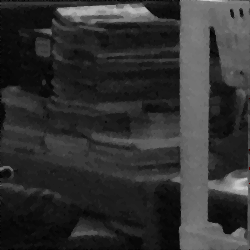
\includegraphics[width=0.5\textwidth]{noiseless_grayscale}
    \caption{Grayscale without noise}
\end{figure}

Ma partie sur le traitement de l’image est ainsi à ce jour constitué de 5 fonctions principales réalisant des taches indispensables pour la reconnaissance de caractère. 

\section{Découpage de l'image (Cédric)}

La première version du découpage de caractère est une version itérative. Elle consiste à parcourir les lignes de l'image jusqu'à trouver un pixel noir indiquant un morceau de caractère (cela nécessite donc que l'image soit traiter au préalable afin d'éliminer les bruits ou bien de choisir des images déjà adaptés). On  garde l'index de la ligne en mémoire puis on continue de parcourir les lignes de l'image jusqu'à ce qu'on tombe sur une ligne sans pixels noirs. On prend l'indice de la ligne précédente qui contenait des pixels en mémoire puis on parcourt les colonnes entre l'intervalle formé par les deux indices mémorisés. La méthode est la même : quand on trouve une colonne contenant un pixel noir on garde l'index de cette colonne en mémoire puis on parcourt les autres jusqu'à trouver une colonne sans pixels noirs, on prend l'index de la colonne précédente et on obtient ainsi 4 bornes qui nous permettent de déterminer un rectangle dans lequel se situe un caractère. On continue ensuite de la même façon à déterminer les caractères en parcourant les autres colonnes. Une fois cela fait on reprend le parcours des lignes en répétant le même processus.

\begin{figure}[H]
    \centering
    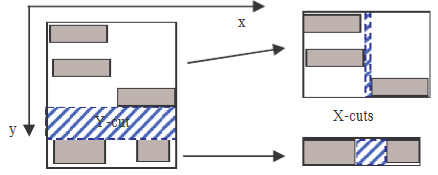
\includegraphics[width=1\textwidth]{Image_segmentation}
    \caption{Image segmentation}
\end{figure}
\vspace{2em}
\begin{figure}[H]
    \centering
    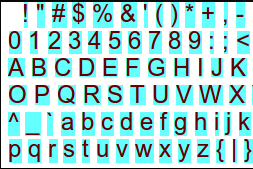
\includegraphics[width=0.8\textwidth]{Seg_example_1}
    \caption{Example 1}
\end{figure}
\begin{figure}[H]
    \centering
    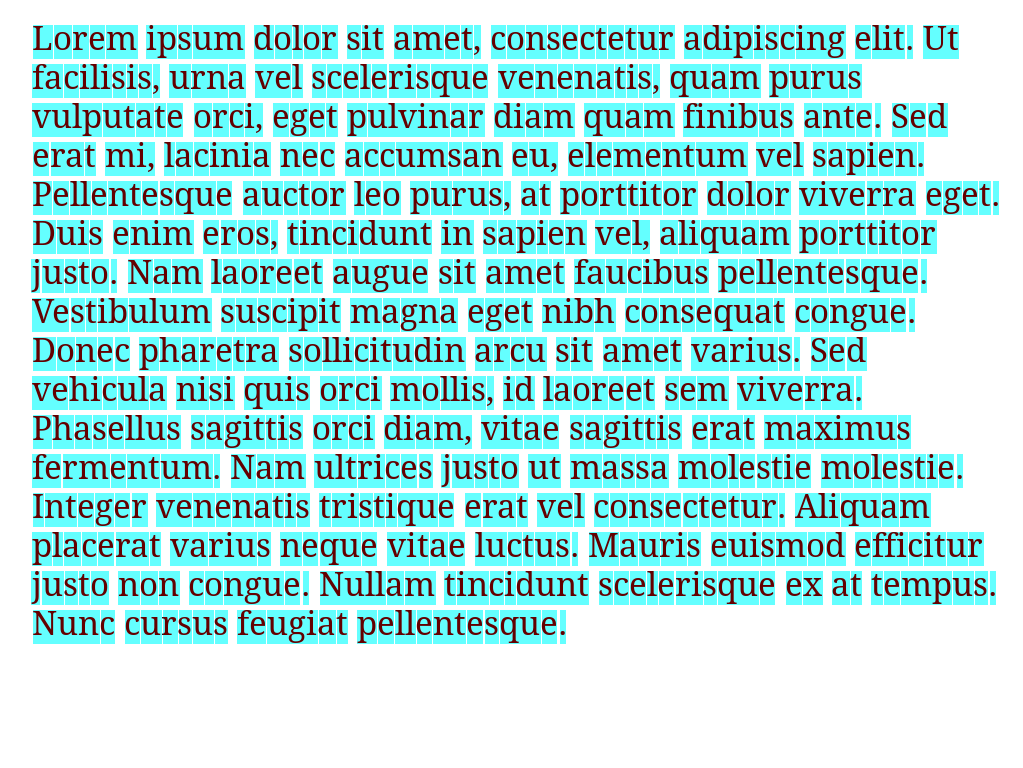
\includegraphics[width=0.8\textwidth]{Seg_example_2}
    \caption{Example 2}
\end{figure}

\newpage
L'objectif avec cette méthode était de pouvoir créer une liste d'image où chaque image correspond à un caractère. On aurait ensuite traiter ces images pour qu'elles aient une taille de 28 pixels par 28 avant de les transformer en matrices pour les donner au réseau de neurones. Un des problèmes qui se montraient était la création d'une liste d'image que l'on n'arrivait pas à implémenter avec SDL. Un autre problème était qu'il n'était pas possible lors de la reconstruction du texte de replacer les espaces et les retours à la ligne.

Des recherches plus poussés nous ont fait savoir que l'utilisation d'une version récursive de la segmentation permettrait de résoudre ce problème notamment grâce au stockage des caractères dans un arbre binaire (qui est une structure récursive). L'algorithme utilisé est le Recursive XY Cut . Il consiste a diviser simultanément le texte horizontalement et verticalement en trouvant les plus grand espaces vides (ici sans caractères) puis de continuer sur les blocs ainsi découper jusqu'à obtenir des blocs sans espaces : les caractères. Cependant l'algorithme seul ne permet pas de réorganiser le texte correctement, nous la modifierons un peu de manière à couper horizontalement jusqu'à ce que cela ne soit plus possible puis de verticalement pour obtenir les caractères dans le bon ordre.

Malheureusement nous étant rendu compte trop tard de l'utilité de la récursion nous n'avons pas eu le temps de finir la segmentation récursive à temps. Seul des fonctions intermédiaires utile pour le découpage ont été codées jusque là.

\newpage
\section{Réseau neuronal (Antoine)}

Pour le réseau de neurones capable d'apprendre la porte logique XOR, je suis partit d'un design classique: 2 entrées, 1 couche cachée contenant 2 neurones, 1 sortie, et 1 biais entre chaque couche. Afin que les données soient organisées, j'ai opté pour des tableaux pour stocker le contenu des noeuds et les poids (les poids entre l'entrée et le \textit{hidden layer} sont nécéssairement stockés dans une matrice). 

Cet algorithme n'a en soit pas grand chose de compliqué. La forward-propagation (résolution de test) revient à additionner le produit des poids par leur entrée, et à stocker la valeur obtenue dans le noeud de sortie auquel les poids sont reliés avant d'appeler la fonction d'activation. La fonction que j'ai choisi est la fonction sigmoïde, suffisante pour un réseau de neuronne de cette taille..

Pour ce qui est de la backward-propagation, il m'a été difficile de réellement saisir le fonctionnement des opérations et surtout comment décomposer le gradient d'erreur. La constante d'apprentissage ETA a été choisie arbitrairement: 0.1. 

Tout cela me donne un réseau qui prend cette forme:

\begin{figure}[H]
    \centering
    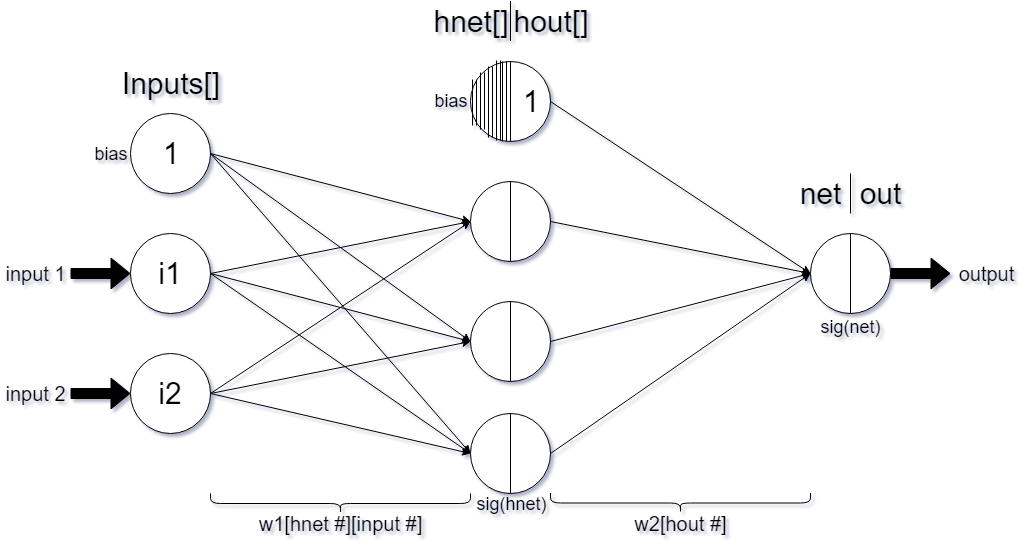
\includegraphics[width=1\textwidth]{XOR_Neural_Network}
    \caption{XOR neural network}
\end{figure}

Mais il ne s'agit ici que du XOR, un \textit{proof of concept}, le \textit{Hello World} des réseaux de neurones. Pour le véritable réseau de notre OCR, il faudra traiter des caractères sous forme d'images de dimensions 28x28 pixels, soit 784 entrées. Il me faudra expérimenter avec le \textit{hidden layer} afin de trouver combien de neuronnes seront nécéssaires, voire s'il est utile d'ajouter une couche supplémentaire. Enfin, pour la sortie, nous allons nous contenter de la reconnaissance des chiffres et des lettres (majuscules et minuscules), soit 62 caractères, donc 62 sorties.

Afin d'entrainer cette future intelligence artificielle, je compte pour le moment utiliser les ressources fournies par NIST dans son \textit{NIST Special Database 19}, disponible à l'adresse suivante: \url{https://catalog.data.gov/dataset/nist-handprinted-forms-and-characters-nist-special-database-19}. 

Je pense qu'une des difficultés principales de la deuxième partie du projet sera d'apprendre à utiliser ces données (en extraire les images et les valeurs attendues), mais cette archive est très complète et contient suffisament d'exemples pour entraîner le réseau de neuronnes.

\section{Interface utilisateur (Jérémy)}

Tout d’abord, je me suis intéressé au choix des bibliothèques qui constitueront notre interface. Nous avons choisi GTK+ pour sa portabilité et est développé à l’origine en C.
Afin d’interagir avec notre application, il nous faut créer une fenêtre. En effet, le widget permettant d’afficher une fenêtre se nomme "GtkWindow". Les objets graphiques utilisent la notion d’héritage afin de récupérer des propriétés et des méthodes d’un widget de ses parents pour modifier leur propre comportement. 

\begin{figure}[H]
    \centering
    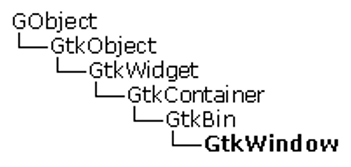
\includegraphics[width=0.5\textwidth]{GTK1}
    \caption{Windows inheritance with GTK}
\end{figure}

Ensuite, nous devions utiliser plusieurs éléments essentiels d’une interface graphique : les box et les boutons. GTK+ a certains avantages comme certains inconvénients. Nous ne pouvons pas intégrer plusieurs widgets dans une fenêtre car un "GtkContainer" ne peut en contenir qu’un seul. Pour résoudre ce problème, je me suis penché sur l’utilisation de deux catégories de "GtkBox" :

\begin{itemize}[label=\textbullet]
	\item Les \textbf{GtkHBox} qui permettent de disposer les widgets horizontalement
	\item Les \textbf{GtkVBox} qui permettent de les disposer verticalement
\end{itemize}

Egalement, les boutons permettent à l’utilisateur d’effectuer une action grâce à un simple clic de souris. 

\begin{figure}[H]
    \centering
    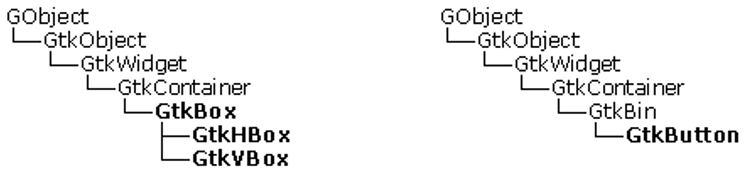
\includegraphics[width=1\textwidth]{GTK2}
    \caption{Boxes and buttons inheritance with GTK}
\end{figure}

Pour cela, j’ai étudié la théorie des signaux afin que ceux-ci ne se terminent qu’au moment où l’utilisateur le demande. Lorsque l’utilisateur interagit avec l’application, le widget concerné émet un signal. Il est associé à un ou plusieurs signaux et permet donc ainsi de programmer toutes les actions possibles. J’ai donc créé plusieurs fonctions "callback" qui connecte le signal au bouton concerné. 
Nous pouvons effectuer plusieurs actions dont les trois premières s’activent avec le signal "clicked":

\begin{itemize}[label=\textbullet]
	\item Ouvrir une image
	\item Ouvrir une zone de texte
	\item Fermer cette zone
	\item Quitter l'application (avec le signal "destroy")
\end{itemize}

J’ai inclus notamment, une barre de défilement pour que le texte converti ne soit pas bloqué par une taille fixe de la zone de texte.
Voici une image montrant l’avancement actuel de l’interface graphique.

\begin{figure}[H]
    \centering
    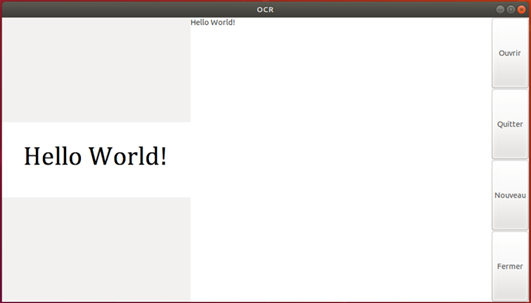
\includegraphics[width=1\textwidth]{UI}
    \caption{Current user interface}
\end{figure}

Enfin, la prochaine étape sera de créer le bouton "Convert". En effet, nous devrons relier l’interface graphique avec toutes les étapes nécessaires à la construction d’un texte (traitement, découpage et réseau neuronal). Sauvegarder celui-ci sera également prévu pour la dernière soutenance.

\chapter{Avances, retards, difficultés rencontrées}

\section*{Traitement de l'image}

Le début du projet fut très difficile pour différentes raisons. Tout d’abord il a fallu apprendre un nouveau langage de programmation : le C. Il a donc fallu se renseigner sur ses spécificités, ses difficultés et ses bibliothèques. De plus ce langage est venu avec énormément de nouveautés pour moi. En effet je n’avais que très peu utilisé les lignes de commande auparavant et encore moins utilisé Vim. J’ai donc appris à utiliser ces nouveaux outils tout en me renseignant sur le C et en commençant à travailler sur ce projet. L'éditeur n’a pas été simple à prendre en main car il demande l’ajout de plusieurs fonctionnalités pour le rendre plus agréable à l’utilisation. De plus ses raccourcis ne sont pas forcément intuitifs et demandent quelques semaines de pratique pour les maitriser. J’ai ensuite lu plusieurs documentations concernant SDL, qui allait devenir très importante pour ma partie. 

Après les premiers travaux pratiques j’ai vite compris qu’il fallait organiser son code en plusieurs fichiers afin d’obtenir un projet lisible et de ne pas perdre de temps lorsque l’on cherche des éléments. J’ai donc pris le temps d’organiser mes fonctions en différents fichiers pour améliorer sa lisibilité. 

Une des parties qui m’a posé le plus de problème a été la compréhension des pointeurs. Les pointeurs sont des outils nouveaux pour moi, je ne savais absolument pas ce que c’était avant de commencer le projet.  

\section*{Découpage de l'image}

Une première difficulté pour moi a été de me familiariser avec le langage C et la librairie SDL. Chercher à créer une liste d'image pour compléter ma segmentation itérative m'a pris du temps et s'est soldé par un échec. M'être rendu compte trop tard qu'une version récursive était probablement une meilleure solution a fait que je me retrouve en retard pour cette première soutenance.

Le point positif est qu'il vaut mieux s'en être rendu compte maintenant et avoir commencé à coder la version récursive plutôt que de s'en rendre compte plus tard et avoir perdu encore plus de temps.

\section*{Réseau neuronal}

Comme dit plus haut, j'ai eu beaucoup de difficultés à comprendre pourquoi le réseau de neuronnes, qui la majorité du temps fonctionne sans problème, n'apprenait parfois pas la moitié de la table de vérité du XOR. Il s'agissait en fait d'un problème de minimum local. N'ayant pas réussi à implémenter de momentum, je me suis contenté de mitiger la probabilité de tomber dans un minimum local en ajoutant un neurone supplémentaire dans la couche cachée.

Pour le réseau de neurone de l'OCR, j'utiliserai simplement un seed prédéfinit pour le random: une valeur d'initialisation de l'aléatoire pour laquelle l'apprentissage fonctionne, car il n'est pas nécéssaire d'avoir un aléatoire différent à chaque apprentissage du réseau, du moment que celui-ci fonctionne.

A cause de ce problème sur lequel j'ai passé trop de temps, je n'ai pas pu commencer à m'occuper de l'enregistrement des poids du réseau neuronal. Il faudra donc mettre cela en place pour la soutenance finale.

Autrement, l'autre difficulté de cette partie a été d'apprendre à utiliser les pointeurs et \textit malloc pour utiliser les tableaux en C.

\section*{Interface utilisateur}

Concernant l’interface graphique, j’ai eu de nombreuses difficultés que j’ai réussi à surmonter. 

En effet, je devais intégrer correctement deux box (l’une étant la zone d’image, l’autre, l’emplacement des boutons) dans un conteneur (appelé "main\_box") qui lui-même se trouve dans une fenêtre. Le tout rendait finalement notre application intuitive.

Egalement, je pensais qu’il fallait contenir un widget image dans une zone de texte. Je me suis rendu compte que ce n’était pas la bonne solution après quelques jours, me tournant vers une option plus pragmatique : créer une nouvelle box.

Ma principale épreuve était de rapidement apprendre à coder en C car j’utilise dans mon interface, des listes chainées et la notion d’héritage.
Enfin, je ne suis ni en retard, ni en avance par rapport à la répartition des taches.

\chapter{À venir}

\begin{itemize}
	\item \textbf{Traitement :} corriger ou adapter le traitement en fonction des besoins après des tests sur le réseau de neuronnes réel.
	\item \textbf{Découpage :} reconstruction du texte. Normalement, l'implémentation récursive permettra une reconstruction simple.
	\item \textbf{Réseau neuronal :} véritable réseau de neuronnes de l'OCR, sauvegarde des poids.
	\item \textbf{Interface :} lier l'interface aux différentes fonctions.
\end{itemize}

\chapter{Expériences personnelles}

\begin{itemize}
	\item \textbf{Louis :} Ce projet me permet personnellement de me forcer à toujours avoir quelque chose à améliorer. Il m’a aussi permis de me familiariser très rapidement avec le C et le terminale. De plus l’entente au sein du groupe est très agréable et me permets de travailler efficacement.
	\item \textbf{Cédric :} Je trouve ce projet intéressant et j'ai envie de mener à bien ma partie même si cela s'annonce beaucoup plus compliqué que ce j'imaginais. Ce projet m'a néanmoins forcé à apprendre Linux et le langage C j'apprécie désormais leur utilisation.
	\item \textbf{Antoine :} Cette première partie du projet a été très intéressante pour moi. Cela m'a permis d'apprendre ce qu'est un réseau neuronal, comment cela fonctionne, et comment en créer un. L'intelligence artificielle n'est plus un concept totalement opaque pour moi, et je comprend désormais ce dont il s'agit. Après avoir traité de simples 0 et 1 pour une porte logique, j'ai hate de créer le réseau qui sera capable de traiter des images de caractères, bien que cela sera difficile à mettre en place.
	\item \textbf{Jeremy :} Ce projet m’a permis pour l’instant, d’apprendre à coder en C plus rapidement qu’en travaux pratiques. J’ai eu l’occasion de découvrir ce qu’est GTK et la manière dont nous pouvons créer une interface graphique. De plus, il s’agit ici de mon deuxième projet informatique en groupe, ce qui est pour moi, très intéressant et très bénéfique construisant mon expérience en tant qu’ingénieur. J’ai eu quelques difficultés, certes, mais ceux-ci me permettent d’être fier quand je parviens à les résoudre. J’ai hâte de pouvoir construire une véritable interface graphique et à contribuer dans ce projet informatique.
\end{itemize}

\chapter{Conclusion}

La première soutenance de projet arrive, et le groupe est satisfait de son travail. Notre réseau de neuronne XOR fonctionne, nous disposons désormais d'outils de traitement d'image qui faciliteront notre travail à venir, le découpage de l'image en lignes puis caractères fonctionne parfaitement, et l'interface utilisateur avance bien. Toutefois, il reste beaucoup de travail, et le plus difficile reste à venir. Le réseau de neurones attendu est beaucoup plus complexe que celui chargé d'apprendre la porte logique XOR, et il faut également l'entrainer. L'interface doit être terminée et reliée aux fonctions de l'OCR au plus vite. Et il faudra probablement corriger l'implémentation du traitement d'images et du découpage en fonction des résultats de futurs tests "en conditions réelles".

Malgré les difficultés rencontrées, le groupe est motivé, et très confiant. Bien que certaines parties vont devenir plus chargées, d'autres vont s'alléger, permettant ainsi aux membres d'aider les autres plus facilement. L'OCR sera donc réalisé dans son entièreté en temps et en heure.

\vfill

%\begin{figure}[H]
%    \centering
%    \includegraphics[width=0.8\textwidth]{project_real_mood}
%\end{figure}

\end{document}
